% !TEX root = ../master-thesis.tex

% \begin{figure}
%     \centering
%     \addletter{85}{a} \phantom{4}
%     \includegraphics[width=1.25in]{imgs/RF.jpg}
%     \hspace{1cm}
%     \addletter{85}{b} \phantom{4}
%     \includegraphics[width=1.25in]{imgs/MW.jpg}
%     \caption{
%         \textbf{RF and MW antennas used for spin control.}
%         (a) PCB-based radiofrequency (RF) antenna used for driving spin transitions at MHz frequencies. 
%         (b) Microwave (MW) loop antenna, designed to efficiently couple to hyperfine transitions in $^6$Li. 
%         These antennas are used for coherent spin manipulation. 
%         % performance characterization via spin-flip fidelity is discussed in the following figures.
%     }
%     \label{fig:rfmw}
% \end{figure}







The UniRand experimental apparatus is designed to realize and investigate complex quantum many-body dynamics using ultracold fermionic $^6$Li atoms. The primary objective of the setup is to create highly controllable initial quantum states, facilitate quantum simulation of the Fermi-Hubbard model, and enable precise measurements of quantum observables, such as entanglement entropy and particle correlations, by employing Random Unitary Protocols \cite{culemann_construction_2024, huang_construction_2024}.

The experimental procedure starts with $^6$Li atoms emitted from an atomic oven. Lithium atoms are first collected and precooled in a two-dimensional magneto-optical trap (2D MOT), effectively capturing a high flux of atoms. From there, the atoms are transferred into a three-dimensional magneto-optical trap (3D MOT) for additional cooling and confinement, reaching temperatures near the Doppler limit (approximately 141~$\mu$K for $^6$Li) \cite{culemann_construction_2024, huang_construction_2024}.


Following the 3D MOT, atoms are loaded into a crossed optical dipole trap (ODT), generated by intersecting laser beams, creating a stable potential. At this stage, evaporative cooling further reduces the temperature significantly below quantum degeneracy conditions, reaching regimes where a molecular Bose-Einstein condensate (mBEC) can form. One of the first tasks within this thesis involved developing software for analyzing mBEC preparation data. Figure~\ref{fig:mbec} illustrates results from this analysis, demonstrating the phase space density (PSD) increasing with reduced temperature due to evaporative cooling (Fig.\ref{fig:mbec}a). Atom density profiles at various temperatures show a characteristic bimodal distribution at low temperatures, indicative of mBEC formation (Fig.\ref{fig:mbec}b). Fitting a Gaussian profile to the thermal wings of this distribution (red points in Fig.\ref{fig:mbec}c) clearly reveals a central peak representing the condensed fraction (blue shaded area in Fig.\ref{fig:mbec}c).

After reaching degeneracy in the ODT, atoms are adiabatically transferred into an optical tweezer array, typically implemented using crossed acousto-optic deflectors (AODs). These tweezers provide deterministic preparation of quantum states with single-site control. Precise atom number management is achieved through the spilling technique, which utilizes a magnetic field gradient and controlled reduction of tweezer depth to selectively retain atoms in low vibrational states \cite{culemann_construction_2024, huang_construction_2024}.

A critical aspect of our experiment is precise atom counting, particularly important when recapturing atoms from tweezers back into the MOT for calibration purposes. Atom number quantization can be clearly observed through fluorescence signal histograms, obtained with prolonged exposure times in a MOT loaded with a small number of atoms. Figure~\ref{fig:spillingadd}a shows discrete peaks corresponding to integer atom numbers, confirming accurate and reliable single-atom counting. 
% Moreover, the measured two-dimensional step plot (Fig.~\ref{fig:spillingadd}b) illustrates how varying tweezer power and magnetic field gradient systematically controls atom number, ensuring high fidelity and repeatability for deterministic state preparation.

Future experimental plans involve transferring precisely prepared atoms into optical lattices engineered to simulate the Fermi-Hubbard model. Lattice depth and geometry, as well as disorder potentials, will be precisely tuned, with disorder introduced using a digital micromirror device (DMD), essential for studying localization phenomena \cite{huang_construction_2024}.

High-resolution, spin-resolved imaging is crucial for detailed characterization of quantum states. Imaging employs fluorescence-based free-space techniques, enabling rapid and high-fidelity spin detection. Atoms are transferred to stretched hyperfine states, optimizing photon collection efficiency through closed cycling transitions.

Control over atomic spin states is executed using dedicated radiofrequency (RF) and microwave (MW) antennas
% , shown in Fig.\ref{fig:rfmw}
. 
The PCB-based RF antenna 
% (Fig.\ref{fig:rfmw}a) 
drives MHz-range spin transitions, while the MW loop antenna 
% (Fig.~\ref{fig:rfmw}b) 
efficiently couples to hyperfine transitions, enabling coherent manipulation critical for state preparation, spin-selective procedures, and precise quantum control.

The entire experimental cycle—including state preparation, evolution, and measurement—is optimized for rapid ( cycle time is about 2s) and reliable repetition, allowing statistically robust data collection. 



\begin{figure}
    \centering
    \addletter{200}{a}
    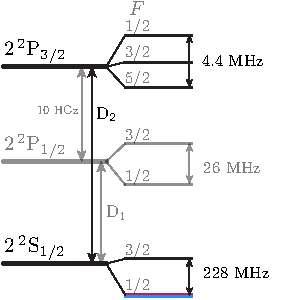
\includegraphics{fig-ai/li-levels-base.pdf}
    \hspace{1cm}
    \addletter{200}{b}
    \includegraphics{fig-ai/li6-zeeman-broken-ai.pdf}
    \caption{
        \textbf{${}^6$Li energy levels}. 
        a) Level diagram of the ground and excited states of ${}^6$Li \cite{gehm_preparation_2003}, including the D1 and D2 transitions around $\lambda = 671$~nm. 
        b) Zeeman splitting of the hyperfine levels of the $2\, {}^2\mathrm{S}_{1/2}$ and $2\, {}^2\mathrm{P}_{2/2}$ in ${}^6$Li \cite{serwane_deterministic_2011, sibalic_arc_2017}. As different spin states for physics we consider state $\ket{1}$ and $\ket{2}$, but for imaging it is worth to flip them to stretched states $\ket{6}$, $\ket{3}$. Colored lines indicate transitions driven by radiofrequency (RF) and microwave (MW) fields.
    }
    \label{fig:li6levels}
\end{figure}




\begin{figure}
    \centering
    \includegraphics{fig-py/atom-counting.pdf}
    \caption{
        Calibration histogram for single-atom counting based on fluorescence signal after after loading to the MOT. Clear quantized peaks correspond to integer atom numbers; the solid red line is a multi-Gaussian fit to the distribution. 
    }
    \label{fig:spillingadd}
\end{figure}

